\section{Лекция. Теорема Гаусса в дифференциальной форме. Теорема Гаусса-Остроградского. Потенциал электрического поля. Теорема о циркуляции}

На прошлой лекции было рассказано про Теорему Гаусса в интегральной форме, однако, в силу недостатка времени, про её дифференциальный аналог было сказано мало слов.

\subsection{Теорема Гаусса в дифференциальной форме}

В векторном анализе вводят понятие \textit{дивергенции вектора}:

\begin{equation}\label{opr1}
\mathrm{div\,} \textbf{A} = \lim_{V \rightarrow 0} \frac{\oint \textbf{A}d\textbf{S}}{V}
\end{equation}

Её можно интерпритировать как поток векторного поля через единичный объем, тогда теорему Гаусса можно записать как:

\colorbox{faded}{\underline{\textbf{Теорема Гаусса в дифференциальной форме}}}

\begin{equation}\label{opr2}
\mathrm{div\,} \textbf{E} = 4\pi\rho 
\end{equation}
где $\rho$ - объемная плотнось заряда

В таком виде теорема чаще применяется, что станет ясно, после понимания смысла дивергенции с математической точки зрения.
Для этого рассмотрим в прямоугольной системе координат выделеный малый объем(иначе говоря прямоугольный параллелепипед) ширины dx, длины dy, высоты dz.

\begin{figure}[!ht]
\centering
 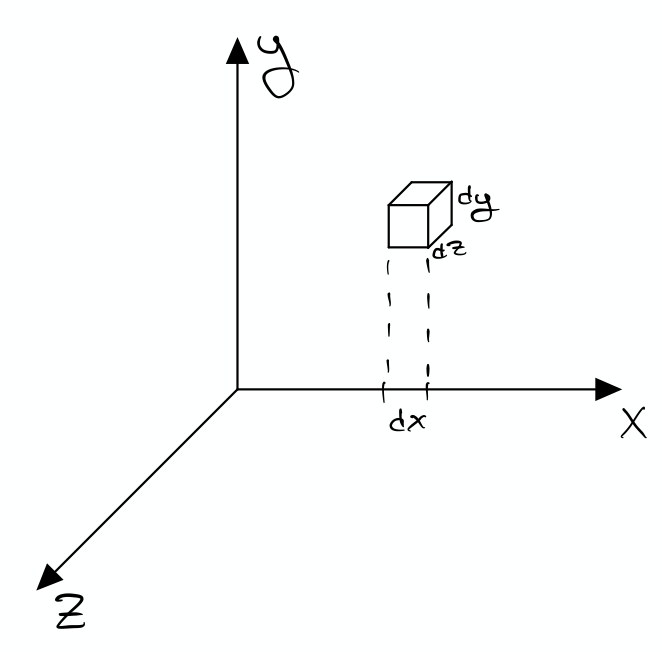
\includegraphics[width=0.4\textwidth]{2_1}     
 \label{fig:my_label}
 \caption{}
\end{figure}

Вычислим разность потоков для одной поверхности 
$$
[E_x(x + dx) - E(x)]dydz = \frac{\partial E_x}{\partial x}dV
$$
Аналогично для других. Отсюда получаем суммарный поток:
$$
\left[\frac{\partial E_x}{\partial x} + \frac{\partial E_y}{\partial y} + \frac{\partial E_z}{\partial z} \right] dV = 4 \pi \rho dV
$$
Следовательно:

\begin{equation}\label{opr3}
\mathrm{div\,}\textbf{E} = \frac{\partial E_x}{\partial x} + \frac{\partial E_y}{\partial y} + \frac{\partial E_z}{\partial z} = \nabla \mathbf{E}
\end{equation}

Используя \textit{\textbf{оператор Набла}}, дивергенцию можно записать как скалярное произведение оператора на вектор-функцию. Учитывая это, справедлива и следующая запись теоремы Гаусса:
\begin{equation}\label{opr4}
\nabla \cdot \textbf{E} = 4 \pi \rho
\end{equation}

\subsection{Теорема Остроградского-Гаусса}
Теорема работает в любом векторном поле (не только в электрическом).

\colorbox{faded}{\underline{\textbf{Теорема Остроградского-Гаусса}}}

\begin{equation}
	\int \mathrm{div} \textbf{A} dV = \oint \textbf{A} d\textbf{S}
\end{equation}

\textit{Интересный вывод}: на поток влияют только заряды на поверхности рассматриваемого объема!

\subsection{Потенциал электростатического поля}

\begin{figure}[!ht]
\centering
 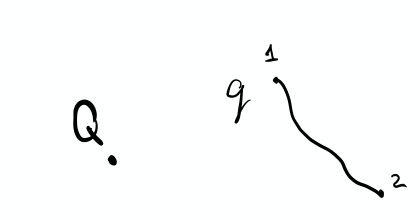
\includegraphics[width=0.4\textwidth]{2_2}     
 \label{fig:my_label}
 \caption{}
\end{figure}

Рассмотрим систему: Заряд $Q$ неподвижен, заряд $q$ находится в точке $1$. Вычислим работу которую нужно совершить для перемещения заряда $q$ из точки $1$ в точку $2$:
\begin{equation}
A_{12} = \int_{1}^{2} q(\textbf{E} d \textbf{r})
\end{equation}

При этом нам известно электрическое поле вдольвсего пути (ф-ла \textit{(1.2)}):
$$\mathbf{E} = \frac{Q}{r^2} \frac{\mathbf{r}}{r}$$

Следователньо:
\begin{equation}
A_{12} = qQ \int_{r_{1}}^{r_{2}} \frac{r ~dr}{r^3} = qQ \left( \frac{1}{r_{1}} - \frac{1}{r_{2}}\right)
\end{equation} 

\textbf{\textit{Вывод:}} работа не зависит от пути, а только от перемещения.

\colorbox{faded}{\underline{\textbf{Опр.}}} \textbf{Потенциал} -- это потенуиальная энергия единичного полодительного заряда. 

\begin{equation}
\varphi = \frac{Q}{r}
\end{equation}

\textit{Примечание:} $\varphi (\infty) = 0$

\colorbox{faded}{\underline{\textbf{Принцип суперпозиции:}}}

\begin{figure}[!ht]
\centering
 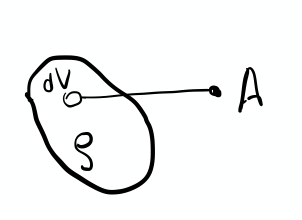
\includegraphics[width=0.4\textwidth]{2_3}     
 \label{fig:my_label}
 \caption{}
\end{figure}

\begin{equation}
\varphi = \sum_{i} \frac{Q_{i}}{r_{i}} = \int_{V} \frac{\rho dV}{r}
\end{equation}

\subsubsection{Теорема о циркуляции}

Данная теорема является следствием всего вышесказанного. \textbf{\textit{Теорема о циркуляции}} гласит:

\begin{equation}
\oint \mathbf{E} d \mathbf{r} = 0
\end{equation}

\colorbox{faded}{\underline{\textbf{Опр.}}} \textbf{Поле потенциально}, если в любой его точке выполнена теорема о циркуляции. А силы в нём \textbf{консервативны}.

\begin{equation}
\mathbf{E} = - \nabla \varphi
\end{equation}

\begin{figure}[!ht]
\centering
 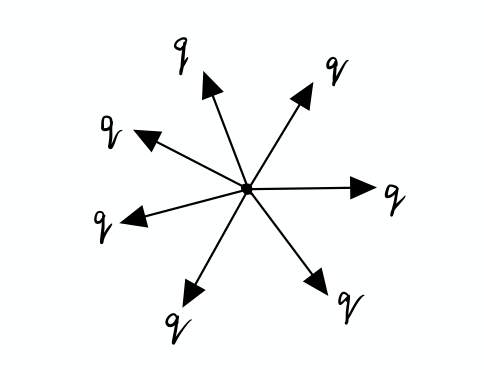
\includegraphics[width=0.4\textwidth]{2_4}     
 \label{fig:my_label}
 \caption{}
\end{figure}

Если бы не выполнялась теорема о циркуляции, то можно было бы построить вечный двигатель. Как бы не мудрили, система не закрутится, так как не может возникнуть силовой линии вихревого характера в силу теоремы о циркуляции.

\textbf{\textit{Байка от Юрия Робертовича:}} Идет экзамен  Студент сдает экзамен профессору. Профессор считает, что студент на нуле, он же наоборот хочет выкарабкаться и просит еще вопросы.\\
Преподаватель: \textit{"Трение -- консервативная сила или нет?"}\\
Преподаватель берет и выбрасывает зачетку за дверь и говорит: \textit{"Если зачетка вернется, я, так и быть, поставлю вам тройку."} В тот момент за дверью проходит студент и пинает зачетку обратно. Пришлось поставить тройку!

\subsubsection{Граничные условия}

Две среды поместили в электрическое поле. Как меняется \underline{тангенциальная составляющая} $E$ при переходе из одной среды в другую? Возьмем контур вдоль границы с очень маленьким расстоянием (так, чтобы можно было пренебречь). Находим циркуляцию. Она должна ровняться нулю. Следовательно (из теоремы о циркуляции):

\begin{equation}
E_{\tau}^{1} = E_{\tau}^{2}
\end{equation}

Что касается \underline{нормальной составляющей}. Легко найти граничные условия по теореме Гаусса:

$S(E_{n}^{1} - E_{n}^{2}) = 4 \pi S \sigma$

\begin{equation}
E_{n}^{1} - E_{n}^{2} = 4 \pi \sigma \text{где} \sigma \text{- заряд на поверхности}
\end{equation}

\begin{figure}[!ht]
\centering
 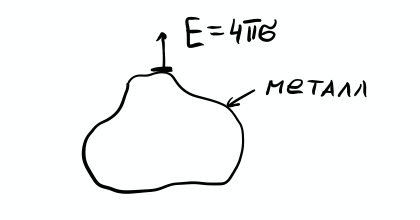
\includegraphics[width=0.4\textwidth]{2_5}     
 \label{fig:my_label}
 \caption{}
\end{figure}

Для металлов: все заряды идут на поверхность. Все заряды распределяются по поверхности. Значит, $\mathbf{E} \perp$ поверхности и равно $E = 4 \pi \sigma$

\subsubsection{Потенциал диполя}

\begin{figure}[!ht]
\centering
 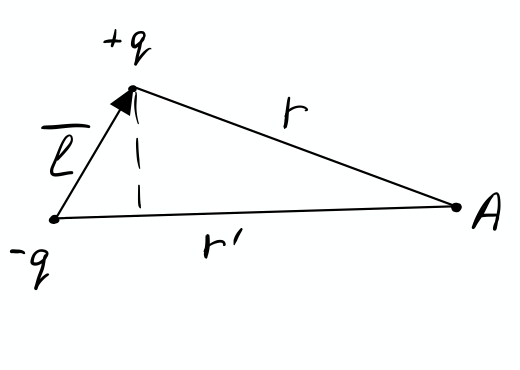
\includegraphics[width=0.4\textwidth]{2_6}     
 \label{fig:my_label}
 \caption{}
\end{figure}

Найдем потенциал точки $A$ по принципу суперпозиции:

$$\varphi = q \left( \frac{1}{r} - \frac{1}{r^{'}} \right)$$

Так как диполь точечный $l \ll r$. Также  $r^{'} = r +l \cos \alpha$.

С учетом всего вышенаписанного и разложения Тейлора \textit{\textbf{потенциал диполя}}:

\begin{equation}
\varphi = \frac{\mathbf{p r}}{r^{3}}
\end{equation}

Ну а \textit{\textbf{напряженность ЭП}}

\begin{equation}
\mathbf{E} = - \nabla \varphi
\end{equation}

\subsection{Теорема о циркуляции в дифференциальной форме. Ротор}

\colorbox{faded}{\underline{\textbf{Теорема о циркуляции в дифференциальной форме}}}

\begin{equation}
\mathrm{rot} \mathbf{E} = 0
\end{equation} 

\colorbox{faded}{\underline{\textbf{Опр.}}} \textbf{Ротор} (для любого поля)

\begin{equation}
rot \mathbf{A} = \lim_{s \rightarrow 0} \frac{\oint \mathbf{A} d \mathbf{S}}{S}
\end{equation} 

\begin{figure}[!ht]
\centering
 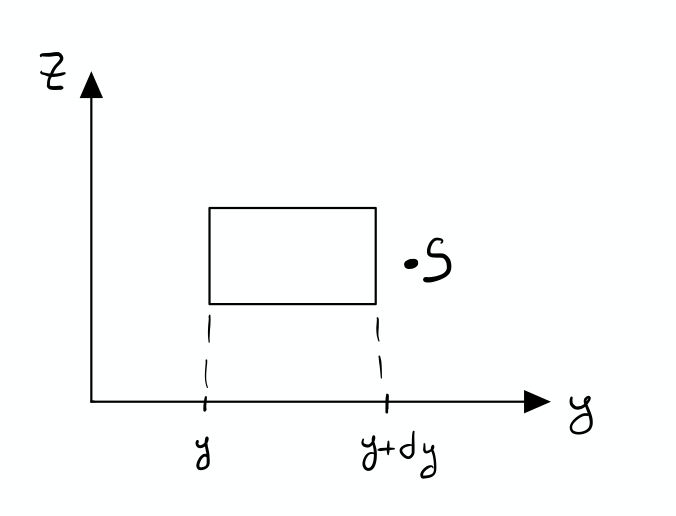
\includegraphics[width=0.4\textwidth]{2_7}     
 \label{fig:my_label}
 \caption{}
\end{figure}

Найдем математическое выражение для ротора. Для этого возьмем ПДКА. Строим прямоугольник. Находим его циркуляцию:

$$(E_{z} (y +dy) - E_{z} (y)) dz = \frac{\partial E_{z}}{\partial y} dy dz$$

Также по другим осям. В результате получим:

$$\mathrm{rot}_{x} \mathbf{E} = \frac{\partial E_{z}}{\partial y} - \frac{\partial E_{y}}{\partial z}$$

$$\mathrm{rot}_{y} \mathbf{E} = \frac{\partial E_{x}}{\partial z} - \frac{\partial E_{z}}{\partial x}$$

$$\mathrm{rot}_{z} \mathbf{E} = \frac{\partial E_{y}}{\partial x} - \frac{\partial E_{x}}{\partial y}$$

\begin{equation}
\Rightarrow \mathrm{rot} \mathbf{E} = \nabla x \mathbf{E} 
\end{equation}

Комментарий к \textit{(2.18)}: векторное произведение для единичной площади $S$

\colorbox{faded}{\underline{\textbf{теорема Стокса}}}

\begin{equation}
\int \mathrm{rot} \mathbf{A} d \mathbf{S} = \oint \mathbf{A} d \mathbf{l}
\end{equation}

\textit{Пояснение:} сумма вихрей внутри зануляется, а значит остается только на поверхности.

\subsection{Уравнение Пуассона и Лапласа}
Еще данные уравнения называют \textit{\textbf{Теоремой ГАуса через потенциал}}.

$$\mathbf{E} = - \nabla \varphi$$

При этом дивергенция:
$$\nabla \nabla \varphi = - 4 \pi \rho$$

\colorbox{faded}{\underline{\textbf{Опр.}}} Лапласиан:
 $$\Delta = \nabla \nabla = \frac{\partial ^2}{\partial x^{2}} + \frac{\partial ^2}{\partial y^{2}}  + \frac{\partial ^2}{\partial z^{2}} $$

Отсюда следует \textbf{\textit{Уравнение Пуассона:}}

\begin{equation}
\Delta \varphi = - 4 \pi \rho
\end{equation}

Если  внутри нет заряда, получаем \textit{\textbf{уравнение Лапласа:}}

\begin{equation}
\Delta \varphi = 0
\end{equation}

\colorbox{faded}{\underline{\textbf{Опр.}}} \textbf{Гармоническая функция} -- функция, удовлетворяющая уравнению Лапласа. Такая функция не имеет максимума и минимума. 

\colorbox{faded}{\underline{\textbf{Теорема единственности}}} 

\begin{figure}[!ht]
\centering
 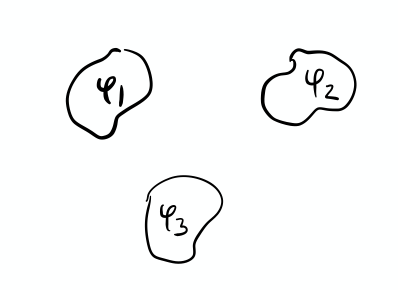
\includegraphics[width=0.4\textwidth]{2_8}     
 \label{fig:my_label}
 \caption{}
\end{figure}

Пусть мы решили уравнение Лапласа, удовлетворив граничным условиям, и получили $\varphi$.

\textit{Доказательство:}

От противного. Пусть существует $\psi$ - решение. Но уравнение Лапласа линейное, значит \\
$\psi^{'} = C_{1} \varphi + C_{2} \psi$ -- удовлетворяет уравнению.

Возьмем:\\
$\psi^{'} = \varphi - \psi$, так как $\varphi$, $\psi$ удовлетворяют условию и в силу гармоничности, и того что на границах $\psi^{'} \equiv -$ получаем $\psi \equiv \varphi  $.

\subsection{Проводники в электрическом поле}

Существуют вещества, являющиеся идеальными проводниками -- \textbf{проводники} (например, медь), а бывают наоборот (например, стекло) -- \textbf{диэлектрики}.

\large
\textbf{\textit{Демонстрация №2.1. "Проводники и диэлектрики"}}.\\
\normalsize

\begin{figure}[!ht]
\centering
 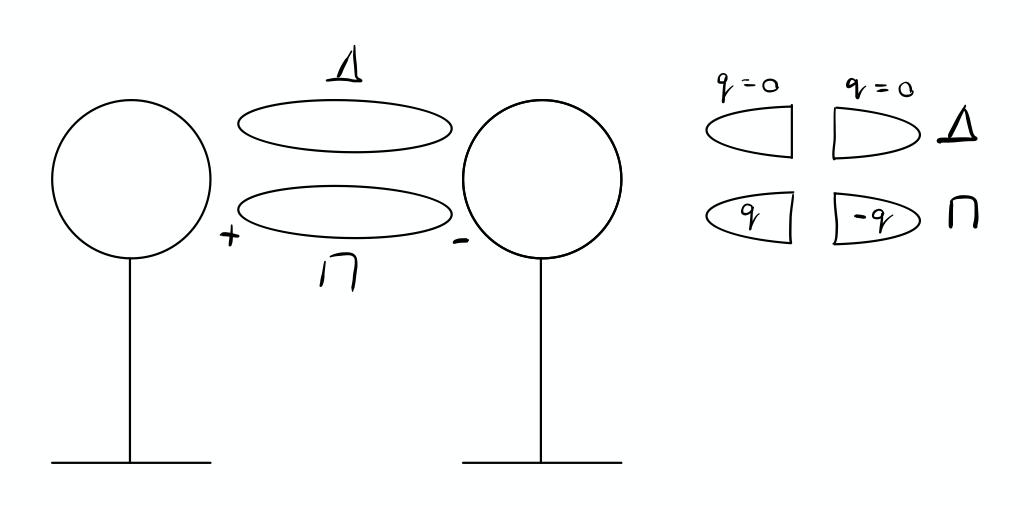
\includegraphics[width=0.4\textwidth]{2_9}     
 \label{fig:my_label}
 \caption{}
\end{figure}

Рассмотрим проводник и диэлектрик в ЭП. Не выключая поле, разрежим проводник и диэлектрик. Далее показано на рисунке.

Хорошими проводниками являются \textbf{металлы}. Внутри них поле равно 0. Иначе заряд переместится на край. Значит, поверхность металла \textit{\textbf{эквипотенциальна}}.

\large
\textbf{\textit{Демонстрация №2.2. "Клетка Фарадея"}}.\\
\normalsize
Видео-демонстрация: \href{https://mipt.lectoriy.ru/lecture/Physics-Coursera-Electricity1-W4D4}{клетка Фарадея}

\large
\textbf{\textit{Демонстрация №2.3. "Звонок Франклина"}}.\\
\normalsize
Видео-демонстрация: \href{https://mipt.lectoriy.ru/lecture/Physics-Coursera-Electricity1-W6D2}{звонок Франклина}

\textit{\textbf{Чем меньше кривизна, тем больше ЭП}}

\textit{Доказательство:}

1. Соединим шары проволокой и зарядим их. Так как конструкция соединина, потенциал должен быть одинаковый. Тогда:

$$\frac{q_{1}}{r_{1}} = \frac{q_{2}}{r_{2}} = \frac{4 \pi r^{2} \sigma_{1}}{r_{1}} = \frac{4 \pi r^{2} \sigma_{2}}{r_{2}}$$

\begin{equation}
\Rightarrow \frac{\sigma_{1}}{\sigma_{2}} = \frac{r_{1}}{r_{2}} = \frac{E_{1}}{E_{2}}
\end{equation}

\begin{figure}[!ht]
\centering
 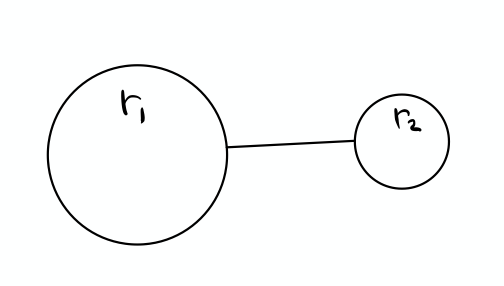
\includegraphics[width=0.4\textwidth]{2_10}     
 \label{fig:my_label}
 \caption{}
\end{figure}


Если взять еталл с острием, тогда возникают очень большие ЭП. Так возникает \textbf{автоэлектронная эмиссия}, когда электроны вылетают. 

\large
\textbf{\textit{Демонстрация №2.4. "Электрический ветер"}}.\\
\normalsize
Видео-демонстрация: \href{https://mipt.lectoriy.ru/lecture/Physics-Coursera-Electricity1-W4D6}{электрический ветер}


